\chapter{Verwendet Technik}

\section{Konzept}
Der Pod wird von einem BLDC-Motor angetrieben, wobei die elektrische Energie in einem Lithium-Ionen-Akku gespeichert wird. Der Motor wird durch einen Sinuswellen-Generator gesteuert. Mit dem Speedgoat-System werden die Eingangssignale des Sinuswellen-Generators sowie andere Aktoren gesteuert.

\section{Antrieb}
\label{Golden_Motor}
Golden Motor ist ein Anbieter von Elektromotoren und elektrischen Antriebssystemen. Das Unternehmen bietet eine breite Palette von Produkten an, darunter:
Motoren und Komplettsysteme für Elektrofahrräder, Industrielle BLDC-Motoren, Elektrische Antriebe für Boote.


\subsection{BLDC Motor}
\label{BLDC_Motor}


Ein BLDC-Motor (Brushless DC Motor) unterscheidet sich grundlegend von einem herkömmlichen Gleichstrommotor. Während bei einem traditionellen DC-Motor die Polumschaltung (Kommutierung) mechanisch über Kohlebürsten erfolgt, übernimmt beim BLDC-Motor eine elektronische Steuerung diese Aufgabe. Dadurch entfällt die Notwendigkeit von Kohlebürsten, was den Motor effizienter und langlebiger macht\cite{mathworks:bldc_motor}.

\begin{figure}[ht]
	\begin{center}
		\includegraphics[width=\textwidth]{img/2_antrieb/motor_1.png}
		\caption{Golden Motors – 10 KW BLDC Motor Liquid Cooled}
		\label{img_2_2:antrieb_motor:1}
	\end{center}
\end{figure}
\pagebreak[4]


Die Anschlüsse des BLDC-Motors sind in Abbildung \ref{img_2_2:circ_bldc:1} dargestellt. Der Motor verfügt über zwei Ausgänge, die jeweils mit drei Hall-Sensoren ausgestattet sind, sowie über einen Temperatursensor. Zusätzlich werden über das Kabel ein GND und eine +5V-Versorgung benötigt. Die Spulen des Motors werden über drei Phasen angeschlossen: U, V und W.

\begin{figure}[ht]
	\begin{center}
		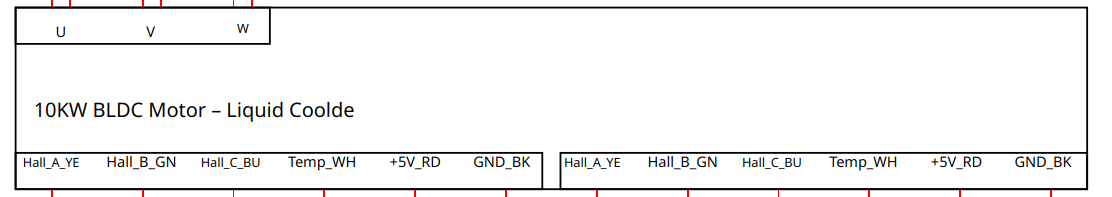
\includegraphics[width=\textwidth]{img/2_imp/2_circ_bldc_motor.png}
		\caption{Zeichnung: BLDC Motor}
		\label{img_2_2:circ_bldc:1}
	\end{center}
\end{figure}
\newpage



\subsection{Vector Controller}
Der Vector Controller verwendet die Motorsteuerungstechnologie feldorientierte Regelung (Field-Oriented Control - FOC), dass bedeutet das der Controller mittels den Hallsensoren, ein Rückgekoppelten Regelkreis bildet und somit die Lage des Polrades ermittelt.

\cite{schroeder:elektische_antriebe}

Sie bietet eine effiziente Steuerung von BLDC-Motoren in Anwendungen mit variabler Drehzahl und schnell wechselnden Lasten und verbessert die Energieeffizienz von Asynchronmotoren, vor allem bei niedrigen Drehzahlen.


\begin{figure}[ht]
	\begin{center}
		\includegraphics[width=\textwidth]{img/2_antrieb/sine_1.png}
		\caption{Golden Motors – VECTOR 500 Motor Controller}
		\label{img_2_2:antrieb_sine:1}
	\end{center}
\end{figure}


%Dafür muss der Abstand ermittelt werden, dies wird mit einem Abstandslaser gemacht.

%Die Steuerung wird als Automaten umgesetzt. Dabei werden unterschiedliche Zustände durchlaufen, wie Idel, Drive, Distance und Stop.
\section{Steuerung}

\begin{figure}[ht]
	\begin{center}
		\includegraphics[width=\textwidth]{img/2_steuerung/goat_1.png}
		\caption{Distanzsensor PEPPERL+FUCHS }
		\label{img_2_2:steuerung_goat:1}
	\end{center}
\end{figure}


\section{Abstandsmessung}

\begin{figure}[ht]
	\begin{center}
		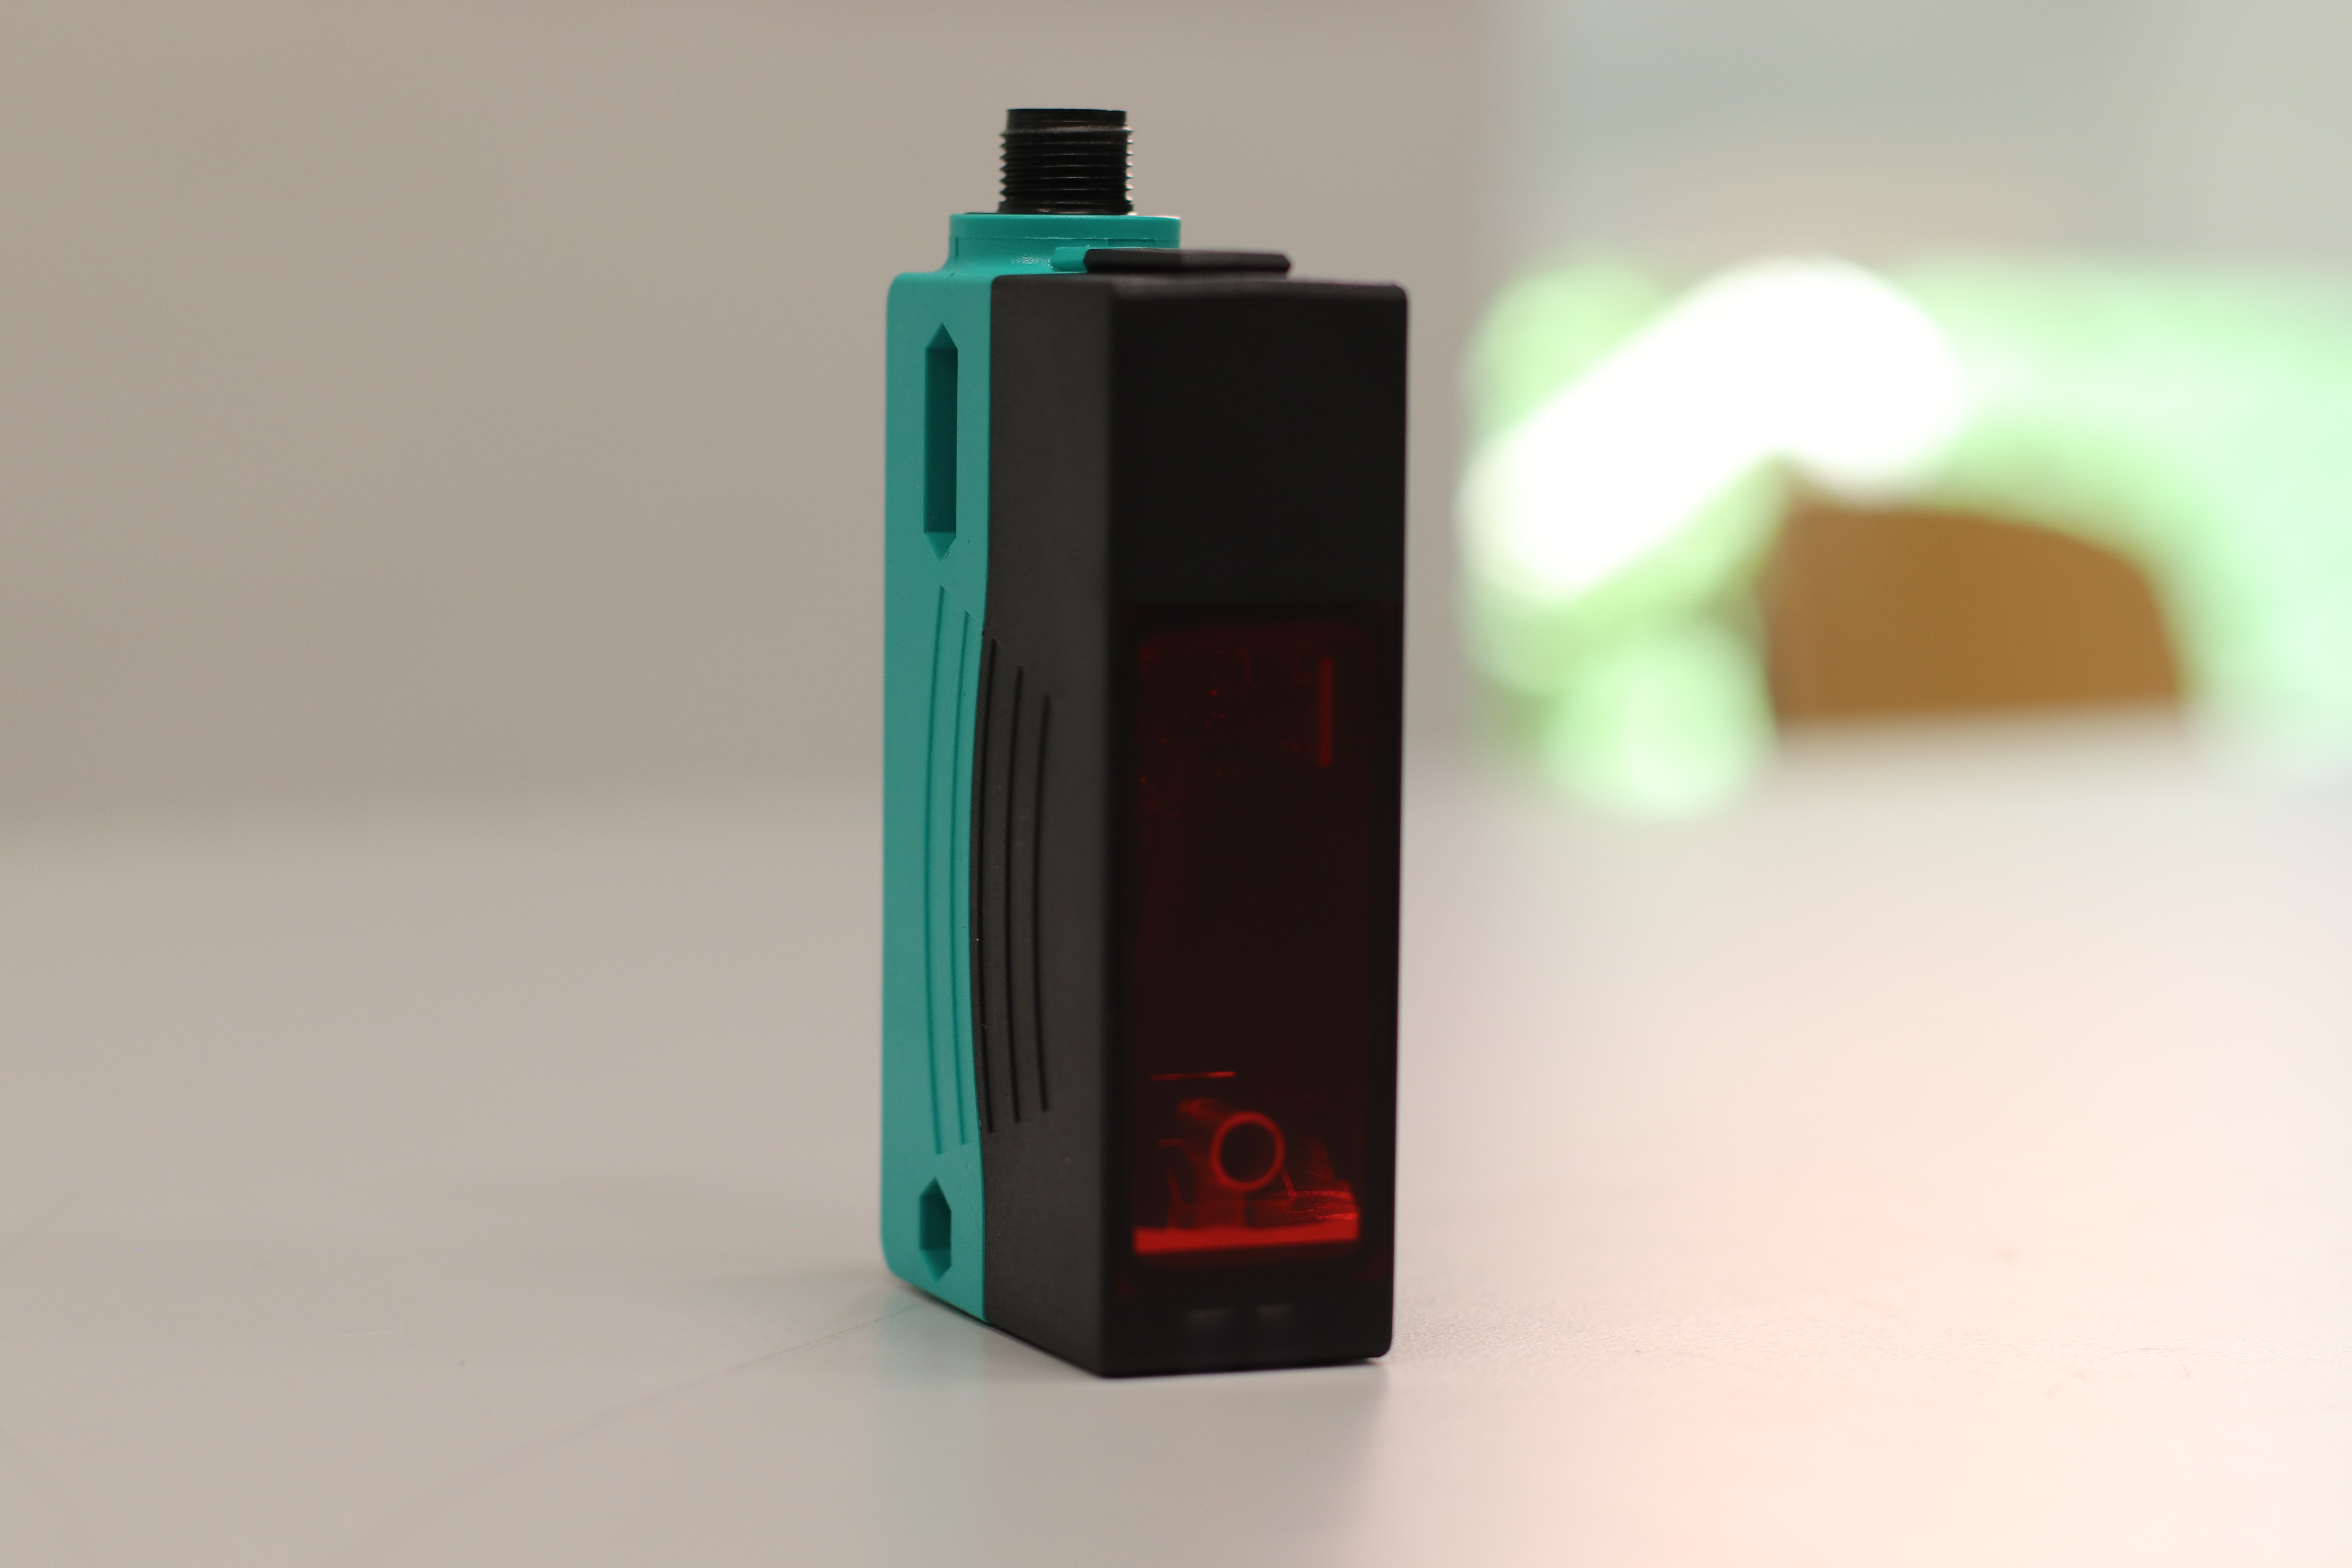
\includegraphics[width=\textwidth]{img/2_sen/dis_1.png}
		\caption{Speedgoat – Baseline Real-Time Target Machine}
		\label{img_2_2:sen_dis:1}
	\end{center}
\end{figure}




\section{Speicher}

\begin{figure}[!ht]
	\begin{center}
		\includegraphics[width=\textwidth]{img/2_speicher/speicher.png}
		\caption{DeepCPower – Lithium Batterie 50Ah | 51,2V | 2560Wh}
		\label{img_2_2:speicher_1:1}
	\end{center}
\end{figure}


